\subsection{SERIES}

Consider a sequence of points \((x_{n})_{n\in \mathbb{N}}\) in a Hausdorff commutative group, and form the sequence of partial sums \(s_n = \sum_{p=0}^{n} x_p (n \in \mathbb{N})\) . The mapping \((x_{n}) \to (s_{n})\) is a bijection of the set \(\mathbf{G}^{\mathbf{N}}\) of sequences \((x_{n})\) of points of \(\mathbf{G}\) , onto itself; for if the sequence \((s_{n})\) is given, the sequence \((x_{n})\) is determined by the relations \(x_{0} = s_{0}, x_{n} = s_{n}-s_{n-1} (n \geqslant 1)\) .

The series defined by the sequence \((x_{n})\) , or the series whose general term is \(x_{n}\) {[}or simply the series \((x_{n})\) , by abuse of language, if there is no risk of confusion{]} is defined to be the pair of sequences \((x_{n})\) and \((s_{n})\) thus associated. The series defined by the sequence \((x_{n})\) is said to be convergent if the sequence \((s_n)\) is convergent; the limit of this sequence is called the sum of the series and is written \(\sum_{n=0}^{\infty} x_n\) (or \(\sum_{n=0}^{\infty} x_n\) , by abuse of notation).

If the series whose general term is \(x_{n}\) is convergent, we shall sometimes allow ourselves, by abuse of language, to refer to it as ``the series \(\sum_{n=0}^{\infty} x_{n}\) '' or ``the series \(x_{0} + x_{1} + \cdots + x_{n} + \cdots\) ''.

A necessary condition for the convergence of the series whose general term is \(x_{n}\) is that the sequence \((s_{n})\) should be a Cauchy sequence, that is to say, that for each neighbourhood V of the origin in G there is an integer \(n_{0}\) such that for each pair of integers \(n \geqslant n_{0}, p > 0\) , we have

\[
s _ {n + p} - s _ {n} = \sum_ {i = n + 1} ^ {n + p} x _ {i} \in V.
\]

If \(\mathbf{G}\) is complete, this condition is also sufficient (Cauchy's criterion for series).

If the series whose general term is \(x_{n}\) is convergent, we have in particular \(\lim_{n\to \infty}(s_n - s_{n-1}) = \lim_{n\to \infty}x_n = 0\) ; but this necessary condition for convergence is by no means sufficient in general, even if \(G\) is complete (see Chapter IV, § 7).

PROPOSITION 7. If the series defined by the sequences \((x_{n})\) and \((y_{n})\) are convergent, then so are the series defined by the sequences \((-x_{n})\) and \((x_{n} + y_{n})\) , and we have

\[
\sum_ {n = 0} ^ {\infty} (- x _ {n}) = - \sum_ {n = 0} ^ {\infty} x _ {n},\tag{7}
\]

\[
\sum_ {n = 0} ^ {\infty} \left(x _ {n} + y _ {n}\right) = \sum_ {n = 0} ^ {\infty} x _ {n} + \sum_ {n = 0} ^ {\infty} y _ {n}.\tag{8}
\]

This is an obvious consequence of the continuity of \(-x\) on \(\mathbf{G}\) , and of \(x + y\) on \(\mathbf{G} \times \mathbf{G}\) .

COROLLARY. If \((x_{n})\) , \((y_{n})\) are two sequences of points of G such that \(x_{n}=y_{n}\) except for a finite number of indices, and if the series whose general term is \(x_{n}\) converges, then so does the series whose general term is \(y_{n}\) .

For the series whose general term is \(x_{n} - y_{n}\) has all its terms zero from a certain index onwards.

This corollary may be put in the form that we may alter arbitrarily a finite number of terms of a convergent series without it ceasing to be convergent. In particular, if \(y_{n} = 0\) for \(n < m\) , and \(y_{n} = x_{n}\) for \(n \geqslant m\) ,

we see that the series whose general term is \(y_{n}\) converges if and only if the series whose general term is \(x_{n}\) converges; its sum is denoted by \(\sum_{n=m}^{\infty} x_{n}\) and is called the residue of index \(m\) of the series \((x_{n})\) . Since

\[
\sum_ {n = m} ^ {\infty} x _ {n} = \sum_ {n = 0} ^ {\infty} x _ {n} - s _ {m - 1},
\]

the residue of index \(m\) of a convergent series tends to o as \(m\) tends to \(+\infty\) .

If a sequence \((x_{n})_{n\in I}\) has as index set an infinite subset \(I\) of \(N\) , and if \(\varphi\) denotes the strictly order-preserving bijection of \(N\) onto \(I\) , then the series defined by the sequence \((x_{\varphi(n)})_{n\in N}\) is called, by abuse of language, the series defined by the sequence \((x_{n})_{n\in I}\) ; if this series is convergent, its sum is denoted by \(\sum_{n\in I}x_n\) . It is immediately verified that this series converges if and only if the series whose general term is \((z_n)\) converges, where \(z_{n}=x_{n}\) if \(n\in I\) and \(z_{n}=0\) if \(n\in G I\) .

\pandocbounded{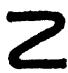
\includegraphics[keepaspectratio]{images/part002_ebf593f8.jpg}}

It is important to notice that if the series defined by a sequence \((x_{n})_{n\in \mathbb{N}}\) converges, there can exist infinite subsets I of \(\mathbf{N}\) such that the series defined by the subsequence \((x_{n})_{n\in \mathbb{I}}\) does not converge (see Exercise 5 and Chapter IV, § 7).

Propositions 4 and 5 extend immediately to series, and we leave their formulation in this case to the reader.

PROPOSITION 8 (Restricted associativity of series). Let \((k_n)\) be a strictly increasing sequence of integers \(\geqslant 0\) . If the series whose general term is \(x_n\) converges, and if we put \(u_n = \sum_{p=k_{n-1}}^{k_n-1} x_p\) , then the series whose general term is \(u_n\) is convergent, and we have \(\sum_{n=0}^{\infty} u_n = \sum_{n=0}^{\infty} x_n\) .

For the sequence of partial sums of the series \((u_{n})\) is a subsequence \((s_{k_{n}-1})\) of the sequence \((s_{n})\) of partial sums of the series \((x_{n})\) .

